
\section{HAR en Android}
\begin{frame}{HAR en Android}

\framesubtitle{Arquitectura del Proyecto}

\setbeamercovered{transparent}
\begin{columns}

\column{0.4\textwidth}
\begin{itemize}
\item \textbf{HARDroid} 
\begin{itemize}
\item Servicio utilitario de reconocimiento.
\item Clasificador din�mico
\end{itemize}

\pause{}
\item \textbf{ActivitySurvey}
\begin{itemize}
\item Aplicaci�n que depende del servicio.
\item Encuesta a usuarios. 
\end{itemize}

\pause{}
\item \textbf{Backend C4.5} 
\begin{itemize}
\item Servicio web de recolecci�n.
\item Aciertos son utilizados para mejorar el clasificador.
\end{itemize}
\end{itemize}

\column{0.6\textwidth}
\begin{center}
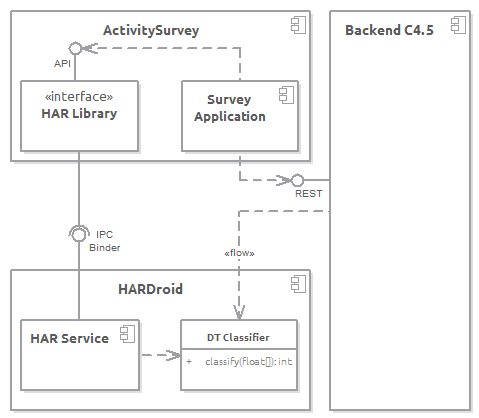
\includegraphics[width=1\columnwidth]{propuesta/graphics/arqui_general}
\par\end{center}

\end{columns}

\end{frame}
%
\begin{frame}{HAR en Android}

\framesubtitle{Servicio de Reconocimiento}

\setbeamercovered{transparent}
\begin{columns}

\column{0.5\textwidth}
\begin{itemize}[<+->]
\item \structure{HARDroid} es un gestor en la capa de \emph{Application Framework}.
\item Mecanismo \structure{IPC} bajo el modelo \structure{Cliente-Servidor}.
\item Las aplicaciones m�viles hechas por terceros obtienen: 
\begin{itemize}
\item mejoras del motor de reconocimiento, 
\item actualizaci�n por plataforma de distribuci�n \structure{Google Play Store}, 
\item mecanismos f�ciles de integraci�n por \structure{Gradle}.
\end{itemize}
\end{itemize}

\column{0.5\textwidth}
\begin{overprint}
\onslide<1-2> 
\begin{center}
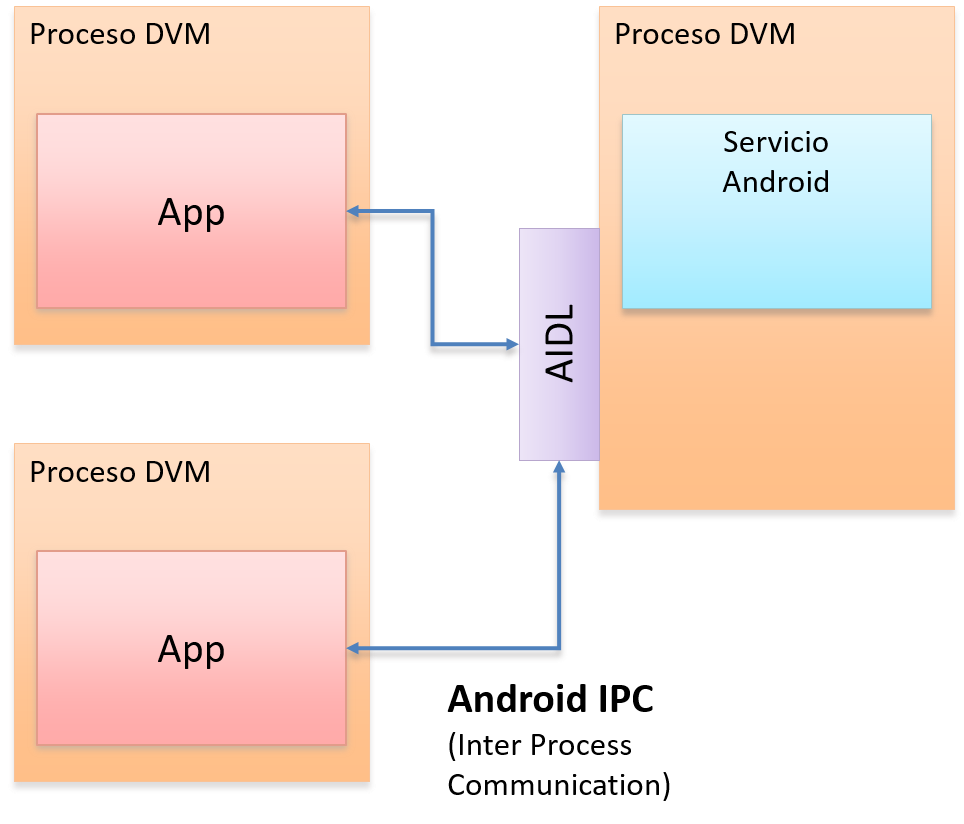
\includegraphics[width=1\columnwidth]{../capitulo-5/graphics/hardroid_func}
\par\end{center}
\onslide<3-> 
\begin{center}
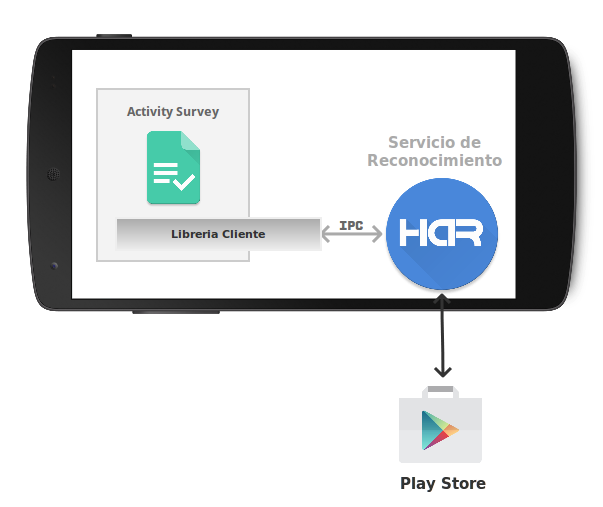
\includegraphics[width=1\columnwidth]{propuesta/graphics/archi_ipc}
\par\end{center}

\end{overprint}
\end{columns}

\end{frame}
%
\begin{frame}{HAR en Android}

\framesubtitle{HARDroid: M�dulos Funcionales}

\setbeamercovered{transparent}
\begin{columns}

\column{0.30\textwidth}
\begin{itemize}[<+->]
\item Integraci�n \structure{AIDL} 
\item Manejo de Sesi�n
\item Procesamiento de muestras
\item Reconocimiento de Actividades
\item Captura de se�ales
\end{itemize}
\begin{center}
\visible<5>{\begin{center}

\includegraphics[width=1.5cm]{propuesta/graphics/hardroid_logo}
\par\end{center}}
\par\end{center}

\column{0.70\textwidth}
\begin{center}
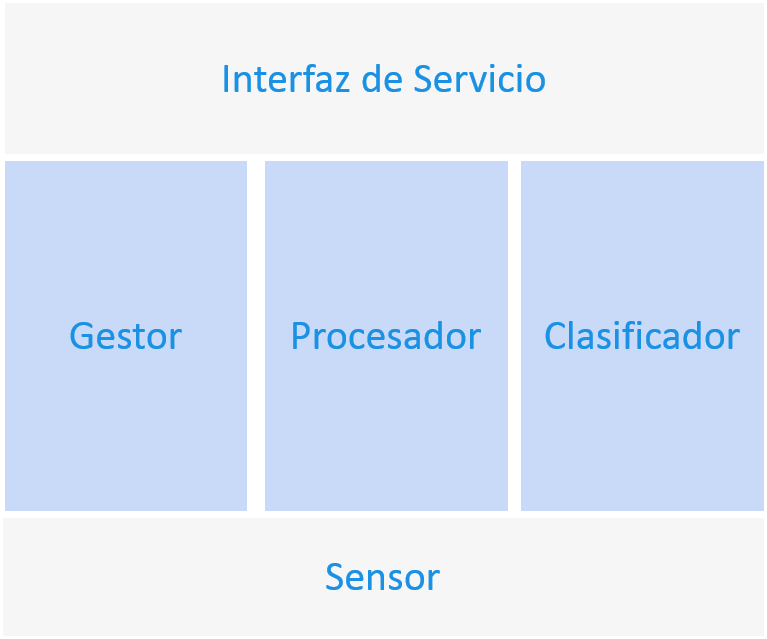
\includegraphics[width=0.9\columnwidth]{propuesta/graphics/hardroid}
\par\end{center}

\end{columns}

\end{frame}
%
\begin{frame}{HAR en Android}

\framesubtitle{Reconocimiento de Actividades}

\centering\resizebox{0.60\textwidth}{!}{%
\noindent\begin{minipage}[t][1\totalheight][b]{1\columnwidth}%
\begin{algorithmic}[1]
    \Require Conjunto de tiempos de subscripci�n de clientes $S$
	\Procedure{Reconocimiento}{$ S $}
		\alertline<1> \If {$S \textit{ est� vac�o } $}
 			\State\textit{Terminar}
		\EndIf 
		\alertline<2> \State $t_w \leftarrow 10$ 
        \Comment{Ventana de tiempo est�ndar de reconocimiento}
		\alertline<3> \State $t_{min} \leftarrow \min_{\forall s \in S} s$
		\alertline<4> \State Esperar $t_{min} - t_w$ segundos 
		\alertline<5> \State $ a_{xyz} = $ Leer sensor por $t_w$ segundos o 512 muestras  
		\alertline<6> {\State $ C = \emptyset$}
		\alertline<7> \For{$i := 1 \to 512$}
			\alertline<8> \State $ v_f = $ Calcular vector caracteristicos de $a_{xyz}$ con valores entre $[i, i + 127]$
			\alertline<9> \State $ c_a = $ Clasificar $v_f$ con el algoritmo \textit{C4.5}
			\alertline<10> \State $ C = C \cup \{c_a\}$
			\alertline<7> \State $i := i + 64$
        \alertline<7> \EndFor
        \alertline<11> \State $ M = $ Calcular matriz de frecuencia de $C$
		\State
		\alertline<11> \Return $ M $
	\EndProcedure
\end{algorithmic}%
\end{minipage}

}
\end{frame}
%
\begin{frame}{HAR en Android}

\framesubtitle{Activity Survey: M�dulos Funcionales}

\setbeamercovered{transparent}
\begin{columns}

\column{0.30\textwidth}
\begin{itemize}[<+->]
\item Presentaci�n
\item Identificaci�n
\item Encuesta guiada
\item Preferencias de comunicaci�n y notificaci�n
\item Almacenamiento y sincronizaci�n
\end{itemize}
\begin{center}
\visible<5>{\begin{center}

\includegraphics[width=1.5cm]{propuesta/graphics/activity_survey_logo}
\par\end{center}}
\par\end{center}

\column{0.70\textwidth}
\begin{center}
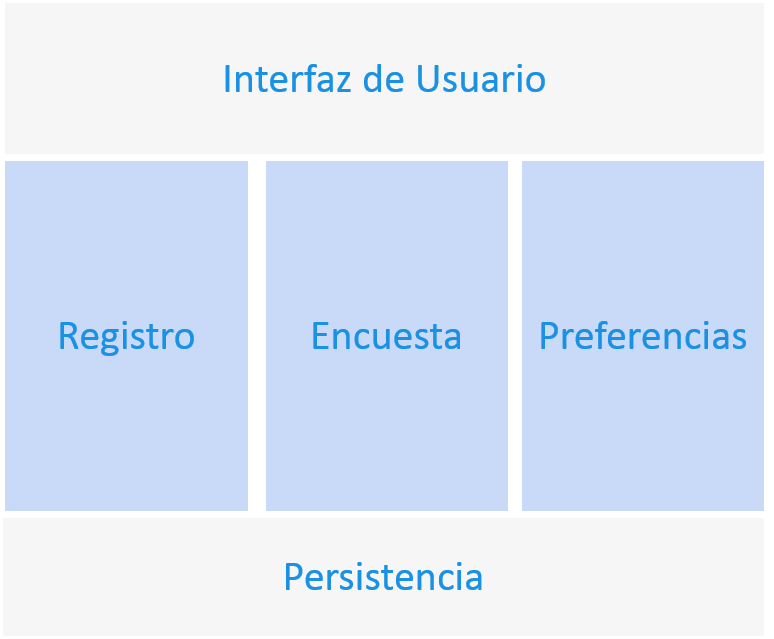
\includegraphics[width=0.9\columnwidth]{propuesta/graphics/activity_survey}
\par\end{center}

\end{columns}

\end{frame}
%
\begin{frame}{HAR en Android}

\framesubtitle{Activity Survey: Componentes Funcionales}
\begin{center}
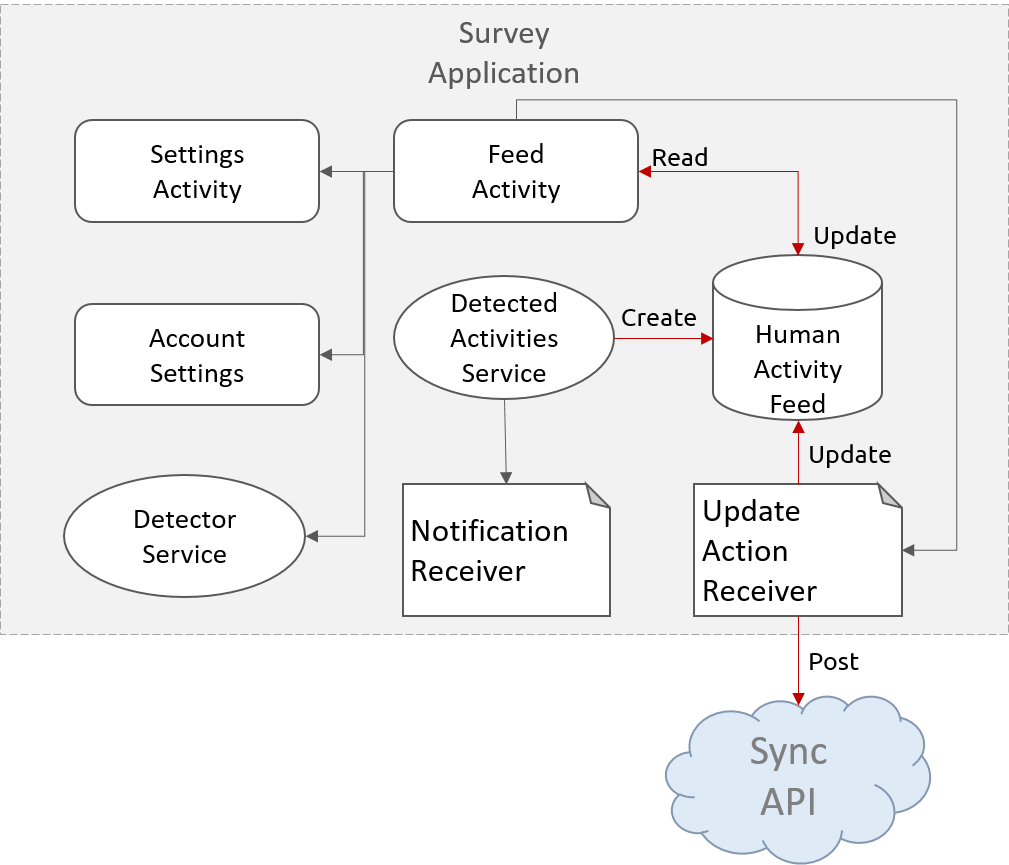
\includegraphics[width=0.65\columnwidth]{../capitulo-5/graphics/act_surv_diag}
\par\end{center}
\end{frame}

